\documentclass{article}
\usepackage[margin=1in]{geometry}
\usepackage[linesnumbered,ruled,vlined]{algorithm2e}
\usepackage{amsfonts}
\usepackage{amsmath}
\usepackage{amssymb}
\usepackage{amsthm}
\usepackage{enumitem}
\usepackage{fancyhdr}
\usepackage{hyperref}
\usepackage{minted}
\usepackage{multicol}
\usepackage{pdfpages}
\usepackage{standalone}
\usepackage[many]{tcolorbox}
\usepackage{tikz-cd}
\usepackage{transparent}
\usepackage{xcolor}
% \tcbuselibrary{minted}

\author{Nathan Solomon}

\newcommand{\fig}[1]{
    \begin{center}
        \includegraphics[width=\textwidth]{#1}
    \end{center}
}

% Math commands
\renewcommand{\d}{\mathrm{d}}
\DeclareMathOperator{\id}{id}
\DeclareMathOperator{\im}{im}
\DeclareMathOperator{\proj}{proj}
\DeclareMathOperator{\Span}{span}
\DeclareMathOperator{\Tr}{Tr}
\DeclareMathOperator{\tr}{tr}
\DeclareMathOperator{\ad}{ad}
\DeclareMathOperator{\ord}{ord}
%%%%%%%%%%%%%%% \DeclareMathOperator{\sgn}{sgn}
\DeclareMathOperator{\Aut}{Aut}
\DeclareMathOperator{\Inn}{Inn}
\DeclareMathOperator{\Out}{Out}
\DeclareMathOperator{\stab}{stab}

\newcommand{\N}{\ensuremath{\mathbb{N}}}
\newcommand{\Z}{\ensuremath{\mathbb{Z}}}
\newcommand{\Q}{\ensuremath{\mathbb{Q}}}
\newcommand{\R}{\ensuremath{\mathbb{R}}}
\newcommand{\C}{\ensuremath{\mathbb{C}}}
\renewcommand{\H}{\ensuremath{\mathbb{H}}}
\newcommand{\F}{\ensuremath{\mathbb{F}}}

\newcommand{\E}{\ensuremath{\mathbb{E}}}
\renewcommand{\P}{\ensuremath{\mathbb{P}}}

\newcommand{\es}{\ensuremath{\varnothing}}
\newcommand{\inv}{\ensuremath{^{-1}}}
\newcommand{\eps}{\ensuremath{\varepsilon}}
\newcommand{\del}{\ensuremath{\partial}}
\renewcommand{\a}{\ensuremath{\alpha}}

\newcommand{\abs}[1]{\ensuremath{\left\lvert #1 \right\rvert}}
\newcommand{\norm}[1]{\ensuremath{\left\lVert #1\right\rVert}}
\newcommand{\mean}[1]{\ensuremath{\left\langle #1 \right\rangle}}
\newcommand{\floor}[1]{\ensuremath{\left\lfloor #1 \right\rfloor}}
\newcommand{\ceil}[1]{\ensuremath{\left\lceil #1 \right\rceil}}
\newcommand{\bra}[1]{\ensuremath{\left\langle #1 \right\rvert}}
\newcommand{\ket}[1]{\ensuremath{\left\lvert #1 \right\rangle}}
\newcommand{\braket}[2]{\ensuremath{\left.\left\langle #1\right\vert #2 \right\rangle}}

\newcommand{\catname}[1]{{\normalfont\textbf{#1}}}

\newcommand{\up}{\ensuremath{\uparrow}}
\newcommand{\down}{\ensuremath{\downarrow}}

% Custom environments
\newtheorem{thm}{Theorem}[section]

\definecolor{probBackgroundColor}{RGB}{250,240,240}
\definecolor{probAccentColor}{RGB}{140,40,0}
\newenvironment{prob}{
    \stepcounter{thm}
    \begin{tcolorbox}[
        boxrule=1pt,
        sharp corners,
        colback=probBackgroundColor,
        colframe=probAccentColor,
        borderline west={4pt}{0pt}{probAccentColor},
        breakable
    ]
    \color{probAccentColor}\textbf{Problem \thethm.} \color{black}
} {
    \end{tcolorbox}
}

\definecolor{exampleBackgroundColor}{RGB}{212,232,246}
\newenvironment{example}{
    \stepcounter{thm}
    \begin{tcolorbox}[
      boxrule=1pt,
      sharp corners,
      colback=exampleBackgroundColor,
      breakable
    ]
    \textbf{Example \thethm.}
} {
    \end{tcolorbox}
}

\definecolor{propBackgroundColor}{RGB}{255,245,220}
\definecolor{propAccentColor}{RGB}{150,100,0}
\newenvironment{prop}{
    \stepcounter{thm}
    \begin{tcolorbox}[
        boxrule=1pt,
        sharp corners,
        colback=propBackgroundColor,
        colframe=propAccentColor,
        breakable
    ]
    \color{propAccentColor}\textbf{Proposition \thethm. }\color{black}
} {
    \end{tcolorbox}
}

\definecolor{thmBackgroundColor}{RGB}{235,225,245}
\definecolor{thmAccentColor}{RGB}{50,0,100}
\renewenvironment{thm}{
    \stepcounter{thm}
    \begin{tcolorbox}[
        boxrule=1pt,
        sharp corners,
        colback=thmBackgroundColor,
        colframe=thmAccentColor,
        breakable
    ]
    \color{thmAccentColor}\textbf{Theorem \thethm. }\color{black}
} {
    \end{tcolorbox}
}

\definecolor{corBackgroundColor}{RGB}{240,250,250}
\definecolor{corAccentColor}{RGB}{50,100,100}
\newenvironment{cor}{
    \stepcounter{thm}
    \begin{tcolorbox}[
        enhanced,
        boxrule=0pt,
        frame hidden,
        sharp corners,
        colback=corBackgroundColor,
        borderline west={4pt}{0pt}{corAccentColor},
        breakable
    ]
    \color{corAccentColor}\textbf{Corollary \thethm. }\color{black}
} {
    \end{tcolorbox}
}

\definecolor{lemBackgroundColor}{RGB}{255,245,235}
\definecolor{lemAccentColor}{RGB}{250,125,0}
\newenvironment{lem}{
    \stepcounter{thm}
    \begin{tcolorbox}[
        enhanced,
        boxrule=0pt,
        frame hidden,
        sharp corners,
        colback=lemBackgroundColor,
        borderline west={4pt}{0pt}{lemAccentColor},
        breakable
    ]
    \color{lemAccentColor}\textbf{Lemma \thethm. }\color{black}
} {
    \end{tcolorbox}
}

\definecolor{proofBackgroundColor}{RGB}{255,255,255}
\definecolor{proofAccentColor}{RGB}{80,80,80}
\renewenvironment{proof}{
    \begin{tcolorbox}[
        enhanced,
        boxrule=1pt,
        sharp corners,
        colback=proofBackgroundColor,
        colframe=proofAccentColor,
        borderline west={4pt}{0pt}{proofAccentColor},
        breakable
    ]
    \color{proofAccentColor}\emph{\textbf{Proof. }}\color{black}
} {
    \qed \end{tcolorbox}
}

\definecolor{noteBackgroundColor}{RGB}{240,250,240}
\definecolor{noteAccentColor}{RGB}{30,130,30}
\newenvironment{note}{
    \begin{tcolorbox}[
        enhanced,
        boxrule=0pt,
        frame hidden,
        sharp corners,
        colback=noteBackgroundColor,
        borderline west={4pt}{0pt}{noteAccentColor},
        breakable
    ]
    \color{noteAccentColor}\textbf{Note. }\color{black}
} {
    \end{tcolorbox}
}


\fancyhf{}
\setlength{\headheight}{24pt}

\date{\today}
\title{Math 115B Homework \#1}

\begin{document}
\maketitle

\begin{prob}
\end{prob}
$T^{-1}$ is linear iff $T^{-1}(w_1+a w_2) = T^{-1}(w_1)+ aT^{-1}(w_2)$ for any $a \in k$ and $w_1, w_2 \in W$. By the definition of an inverse and by the linearity of $T$,
\begin{align*}
    T(T^{-1}(w_1+aw_2)) &= w_1+aw_2 \\
                        &= T(T^{-1}(w_1))+a T(T^{-1}(w_2)) \\
                        &= T(T^{-1}(w_1)+aT^{-1}(w_2)).
\end{align*}
Any invertible function has to be injective, so we can cancel $T$ from both sides, which leaves
\[ T^{-1}(w_1+aw_2)=T^{-1}(w_1)+aT^{-1}(w_2). \]
Therefore $T^{-1}$ is linear.

\bigskip
\begin{prob}
\end{prob}
That is not possible. Suppose $v_1$, $v_2$, and $v_3$ are linearly independent, but $v_1+v_2$, $v_2+v_3$, and $v_3+v_1$ are linearly dependent. Then there exist constants $a_1, a_2, a_3$ which are not all zero, for which
\[ a_1(v_1+v_2)+a_2(v_2+v_3)+a_3(v_3+v_1)=0. \]
This can be rewritten as
\[ (a_3+a_1)v_1+(a_1+a_2)v_2+(a_2+a_3)v_3=0, \]
and since the vectors $v_1$, $v_2$, and $v_3$ are independent, that means $a_3+a_1$, $a_1+a_2$, and $a_2+a_3$ are all zero. However,
\begin{align*}
    a_1 &= (a_3+a_1)+(a_1+a_2)-(a_2+a_3)=0+0-0=0 \\
    a_2 &= (a_1+a_2)+(a_2+a_3)-(a_3+a_1)=0+0-0=0 \\
    a_3 &= (a_2+a_3)+(a_3+a_1)-(a_1+a_2)=0+0-0=0.
\end{align*}
This contradicts our earlier statement, that $a_1$, $a_2$, and $a_3$ are not all zero. Therefore it is not possible.

\bigskip
\begin{prob}
\end{prob}
$k$ contains at least two distinct elements, 1 and 0, so if $V$ were not finite dimensional, $V$ would have infinitely many elements. Therefore $V$ is isomorphic to $k^d$, for some nonnegative integer $d$, so $49=\abs{V}=\abs{k}^d$. This equation is only satisfied if $\abs{k}=7$ and $d=2$, or if $\abs{k}=49$ and $d=1$. In either case, $k$ is finite and $k^d$ is finite-dimensional (with dimension either 1 or 2), which means $V$ also has dimension 1 or 2.

\bigskip
\begin{prob}
\end{prob}
\begin{enumerate}[label=(\alph*)]
    \item For any $w_1 \in W_1$, let $w_2=0$. Since every subspace contains the zero element, $w_2$ is in $W_2$, which means $w_1 + w_2 \in W_1 + W_2$. But $w_1 = w_1+0=w_1+w_2$, so every $w_1 \in W_1$ is also in $W_1+W_2$. This means $W_1 \subset W_1+W_2$, and by the same logic, $W_2$ is also a subset of $W_2+W_1$.
    \item $W_1+W_2$ is clearly a subset of $V$, since $V$ is closed under addition and scalar multiplication, so I only need to show two things: that $W_1+W_2$ is closed under addition, and that it's closed under scalar multiplication. For any $u_1+u_2, v_1+v_2 \in W_1+W_2$, we have $(u_1+u_2)+(v_1+v_2) = (u_1+v_1)+(u_2+v_2)$, which is in $W_1+W_2$ because $u_1+v_1$ is in $W_1$ and $u_2+v_2$ is in $W_2$.
        \par
        $W_1+W_2$ is closed under scalar multiplication, because for any scalar $a$ and vector $w_1+w_2 \in W_1+W_2$, $a(w_1+w_2)=aw_1+aw_2$ is in $W_1+W_2$ because $aw_1 \in W_1$ and $aw_2 \in W_2$.
    \item $W$ is a subspace of $V$, so $W$ is also a vector space over $k$. That means you can just take my answer to part (b) and replace $V$ with $W$.
\end{enumerate}


\bigskip
\begin{prob}
\end{prob}
\begin{enumerate}[label=(\alph*)]
    \item This is a functional, because if $k:=\R$ (or $V=k[x]$), then $f: V \rightarrow k$ and we also have
        \begin{align*}
            f(p+cq) &= 4(p+cq)'(0)+(p+cq)''(1) \\
                    &= (4p'(0)+p''(1))+c(4q'(0)+q''(1)) \\
                    &= f(p)+cf(q).
        \end{align*}
        for any $p, q \in \R[x], c \in \R$.
    \item Not a functional, because the output of $f$ is not an element of $k$.
    \item This is a functional, because $\tr$ is a function from $V$ to $k$, and for any $A,B \in k^{2 \times 2}$ and any $c \in k$,
        \begin{align*}
            f(A+cB) &= \tr(A+cB) \\
                    &= (A+cB)_{1,1}+(A+cB)_{2,2} \\
                    &= (A_{1,1}+A_{2,2})+c(B_{1,1}+B_{2,2}) \\
                    &= \tr(A)+c\tr(B) \\
                    &= f(A)+cf(B).
        \end{align*}
    \item This is a functional. Just like in part (a), I will assume $k := \R$(or $V=k[x]$), so $f: V \rightarrow k$. $f$ is linear because for any $p,q \in V, c \in k$,
        \begin{align*}
            f(p+cq) &= \int_0^1 (p+cq)(x) \d x \\
                    &= \left( \int_0^1 p(x) \d x \right) + c \left( \int_0^1 q(x) \d x \right) \\
                    &= f(p)+cf(q).
        \end{align*}
    \item Not a functional, because
        \[ f \left( \begin{bmatrix}
            1 \\
            0 \\
            0
        \end{bmatrix} + \begin{bmatrix}
            1 \\
            0 \\
            0
    \end{bmatrix} \right) \neq f \left( \begin{bmatrix}
        2 \\
        0 \\
        0
    \end{bmatrix} \right). \]
        
\end{enumerate}


\bigskip
\begin{prob}
\end{prob}
\begin{enumerate}[label=(\alph*)]
    \item Since we already know $\R[x]_{\leq n}$ is a vector space, we just need to show that $W$ is a subspace. If $f, g \in W$ and $c \in \R$, then for any $i \in \left\{ 1,2, \dots, m \right\}$,
        \[ (f+cg)(x_i)=f(x_i)+cg(x_i)=0+0c=0. \]
        By the definition of $W$ and the fact that $\R[x]_{\leq n}$ is a vector space, that means $f+cg \in W$. Since $W$ is a subspace of a vector space over $\R$, $W$ is also a vector space over $\R$.
    \item Let $A: \R[x]_{\leq n} \rightarrow \R^m$ be the function defined by
        \[ A(f) = \begin{bmatrix}
            f(x_1) \\
            f(x_2) \\
            \vdots \\
            f(x_m)
        \end{bmatrix}. \]
        This is clearly a linear map. Since $W := \ker(A)$, the rank-nullity theorem says
        \[ \dim(W) = \dim(V) - \dim(\im(A)) = (n+1) - \dim(\im(A)). \]
        The last step for this problem is to show when $A$ is surjective. For any basis element $e_i$ of $\R^m$, let
        \[ f_i(x) = \prod_{j \in \left\{ 1,2,\dots,m \right\} \backslash \left\{ i \right\}} (x-x_j). \]
        $f_i$ is a degree $m-1$ polynomial, so $f_i \in W$ iff $m-1 \leq n$. If $m > n+1$, then by the fundamental theorem of algebra, $W=\{0\}$, which means $\im(A)$ is also the zero vector space. If $m \leq n+1$, then $f_i \in W$, and $A(f_i)$ is a nonzero scalar multiple of the basis vector $e_i$. In this case, all basis vectors of $\R^m$ are in $\im(A)$, so $\im(A) \cong \R^m$.
        \par
        The image of $A$ is zero-dimensional if $m > n+1$ and $m$-dimensional if $m \leq n+1$, so
        \[ \dim(W) = n+1-\dim(\im(A)) = \max(0, n+1-m). \]
\end{enumerate}


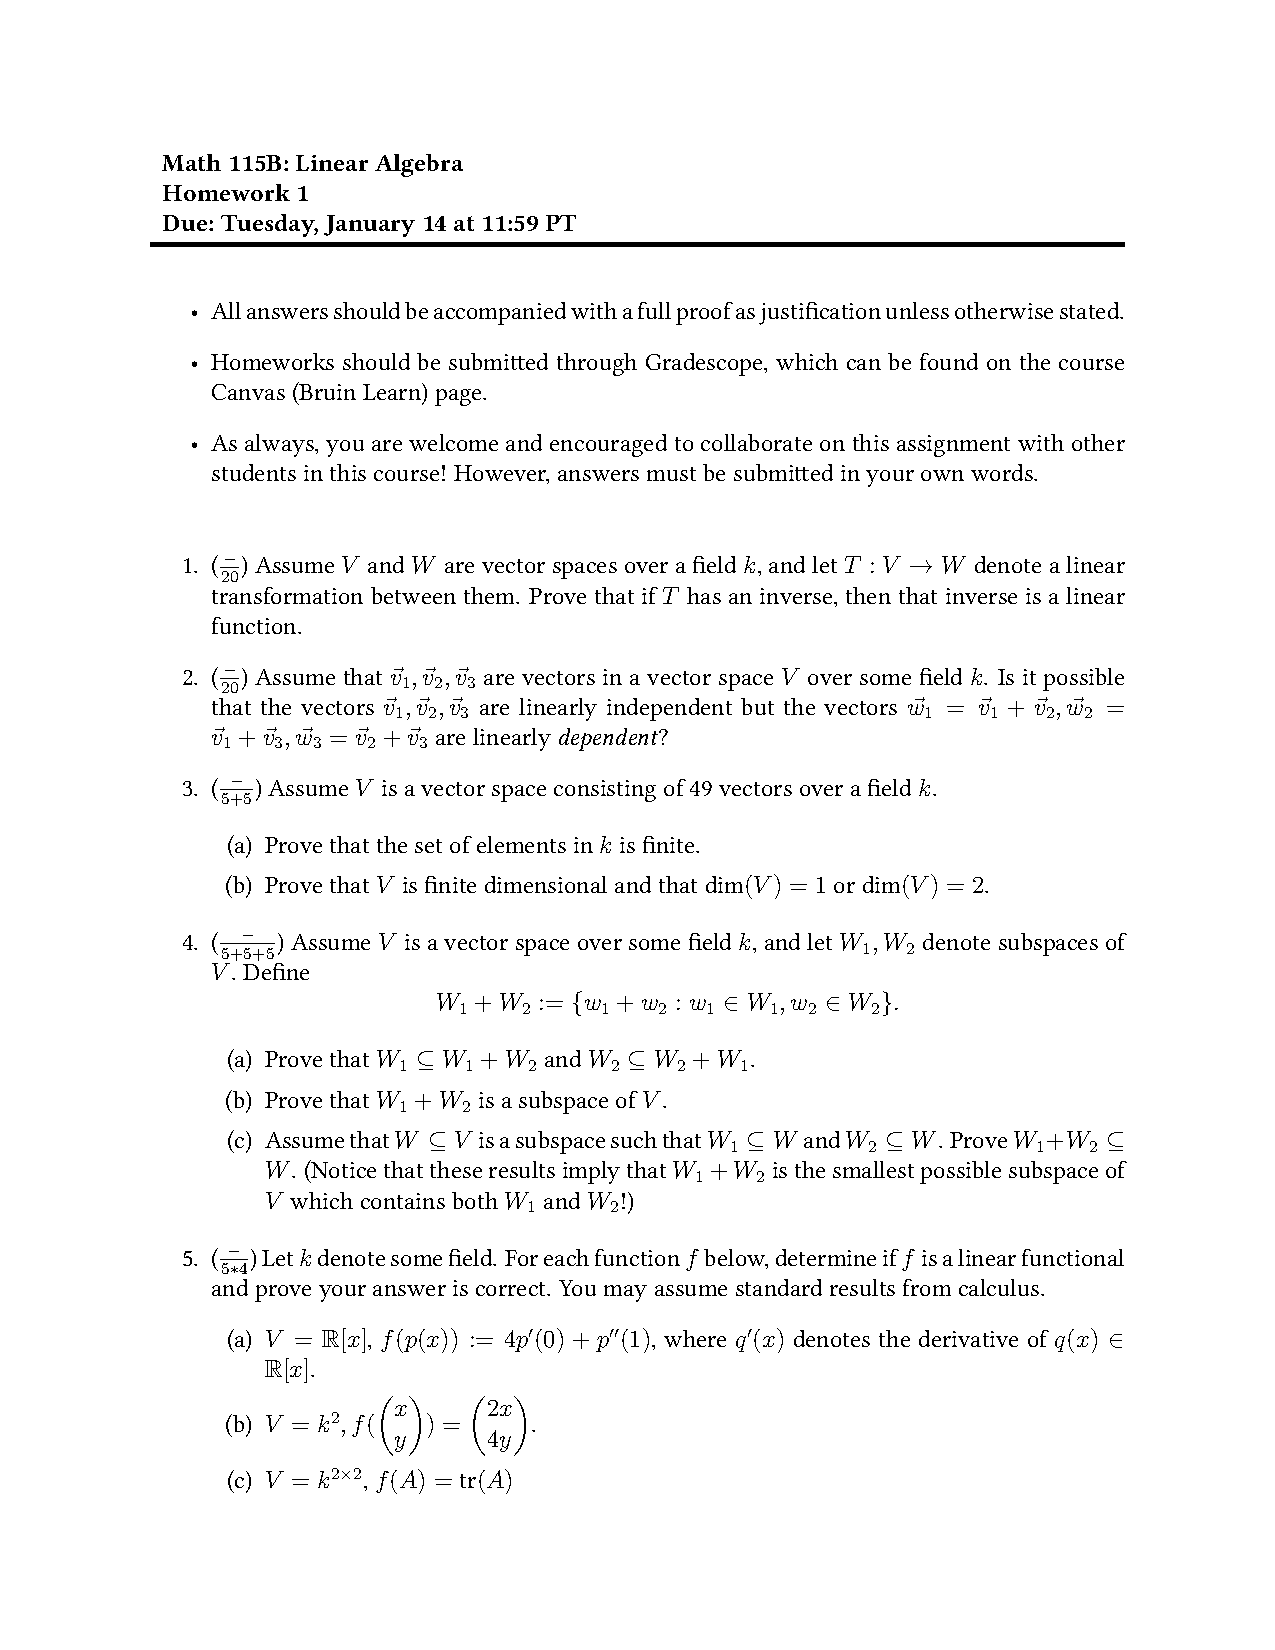
\includepdf[pages=-]{assignment.pdf}

\end{document}
